% Diapositivas de Steven Pozo - avance Día 1

\begin{frame}{Arquitectura: vista respaldada por evidencia}
  \begin{columns}[T]
    \begin{column}{0.62\textwidth}
      \centering
      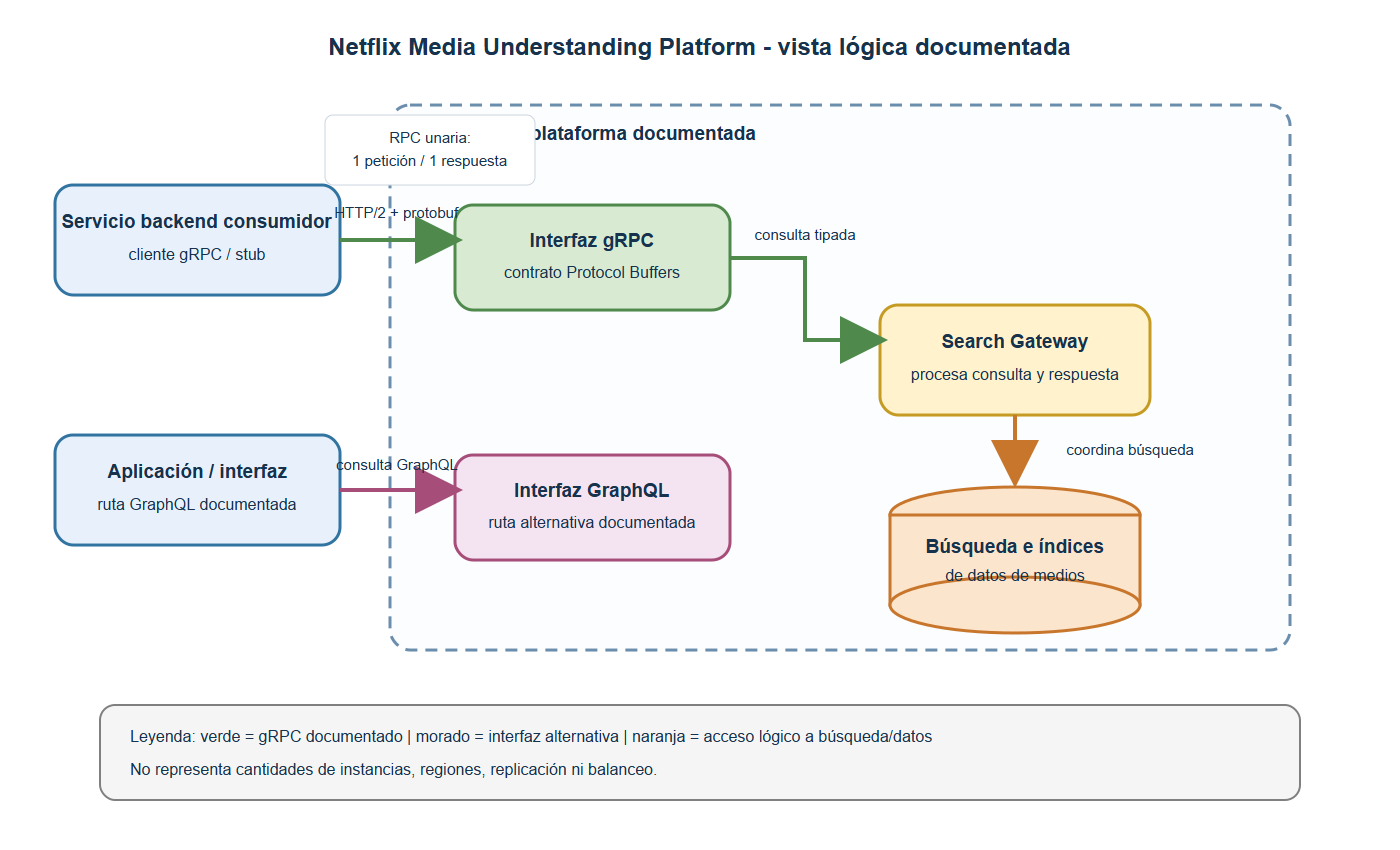
\includegraphics[width=\linewidth]{figuras/arquitectura.png}
    \end{column}
    \begin{column}{0.36\textwidth}
      \begin{itemize}
        \item Caso: Media Understanding Platform
        \item Cliente gRPC: servicio backend consumidor
        \item La aplicación final usa la ruta GraphQL mostrada
        \item Search Gateway coordina consultas
        \item Vista lógica, no topología física completa
      \end{itemize}
    \end{column}
  \end{columns}
  \vfill
  {\tiny Fuente: Netflix Technology Blog (2023), ``Building a Media
  Understanding Platform for ML Innovations''.}
\end{frame}

\begin{frame}{Modelo cliente-servidor y RPC unaria}
  \begin{block}{Una invocación remota}
    Backend cliente / stub $\rightarrow$ una petición protobuf $\rightarrow$ servicio
    gRPC $\rightarrow$ una respuesta o estado.
  \end{block}
  \begin{itemize}
    \item Contrato de servicio definido con Protocol Buffers.
    \item Transporte habitual de gRPC: HTTP/2.
    \item Generación de clientes para varios lenguajes.
    \item La red sigue siendo visible: latencia, deadline y errores.
  \end{itemize}
  \begin{alertblock}{Límite de la afirmación}
    gRPC no garantiza por sí solo replicación, disponibilidad, consistencia ni
    recuperación ante fallos.
  \end{alertblock}
  \vfill
  {\tiny Fuentes: documentación oficial de gRPC; caso de estudio CNCF/Netflix.}
\end{frame}

\begin{frame}{Secuencia de una RPC unaria}
  \begin{enumerate}
    \item El cliente invoca un método del \textbf{stub}.
    \item gRPC serializa una petición con \textbf{Protocol Buffers}.
    \item El servidor ejecuta la operación solicitada.
    \item Regresa una respuesta y un estado, o un error.
  \end{enumerate}
  \begin{block}{Regla para recordarla}
    Invocar $\rightarrow$ serializar $\rightarrow$ ejecutar $\rightarrow$ responder.
  \end{block}
  \begin{alertblock}{No es una función local}
    La llamada cruza la red: puede tener latencia, superar su plazo o fallar.
  \end{alertblock}
  \vfill
  {\tiny Fuente: documentación oficial de gRPC, ``Core concepts, architecture
  and lifecycle''.}
\end{frame}
